\documentclass{article}
\usepackage[portuguese]{babel}
\usepackage[utf8]{inputenc}
\usepackage{makeidx}
\usepackage{graphicx}
\usepackage{fancyhdr}
\usepackage{enumerate}
\usepackage{indentfirst}
\usepackage[a4paper, total={16cm, 24cm}]{geometry}
%---------------------------------------------------------------%
\usepackage{listings}
\usepackage{xcolor}
\definecolor{pblue}{rgb}{0.13,0.13,1}
\definecolor{pgreen}{rgb}{0,0.5,0}
\definecolor{pred}{rgb}{0.9,0,0}
\definecolor{pgrey}{rgb}{0.46,0.45,0.48}
\definecolor{gray}{rgb}{0.4,0.4,0.4}
\definecolor{darkblue}{rgb}{0.0,0.0,0.6}
\definecolor{cyan}{rgb}{0.0,0.6,0.6}
\usepackage{inconsolata}
\lstset{
    language=Java, %% Troque para PHP, C, Java, etc... bash é o padrão
    basicstyle=\ttfamily\small,
    numberstyle=\footnotesize,
    numbers=left,
    backgroundcolor=\color{gray!10},
    frame=single,
    tabsize=2,
    rulecolor=\color{black!30},
    title=\lstname,
    escapeinside={\%*}{*)},
    commentstyle=\color{pgreen},
    keywordstyle=\color{pblue},
    stringstyle=\color{pred},
    breaklines=true,
    breakatwhitespace=true,
    framextopmargin=2pt,
    framexbottommargin=2pt,
    extendedchars=false,
    inputencoding=utf8,
    literate={á}{{\'a}}1 {ã}{{\~a}}1 {é}{{\'e}}1 {ç}{{\c{c}}}1,
}

%---------------------------------------------------------------%
\fancypagestyle{indice}{
\fancyhf{}
\lhead{
\includegraphics[scale=0.3]{imagens/logo.png} }
\rhead{U.C. Estrutura de Dados e Algoritmos II\\
\textbf{1º Trabalho-Mosaics}}
}
%---------------------------------------------------------------%
\pagestyle{fancy}
\fancyhf{}
\lhead{
\includegraphics[scale=0.3]{imagens/logo.png} }
\rhead{U.C. Estrutura de Dados e Algoritmos II\\
\textbf{1º Trabalho-Mosaics}}
\rfoot{\thepage}
\setlength{\headheight}{1.5cm}
%---------------------------------------------------------------%
\title{ 
\includegraphics[scale=0.3]{imagens/uevora.png}\\
U.C. Estrutura de Dados e Algoritmos II\\
\textbf{1º Trabalho-Mosaics \\\vspace{1cm}}
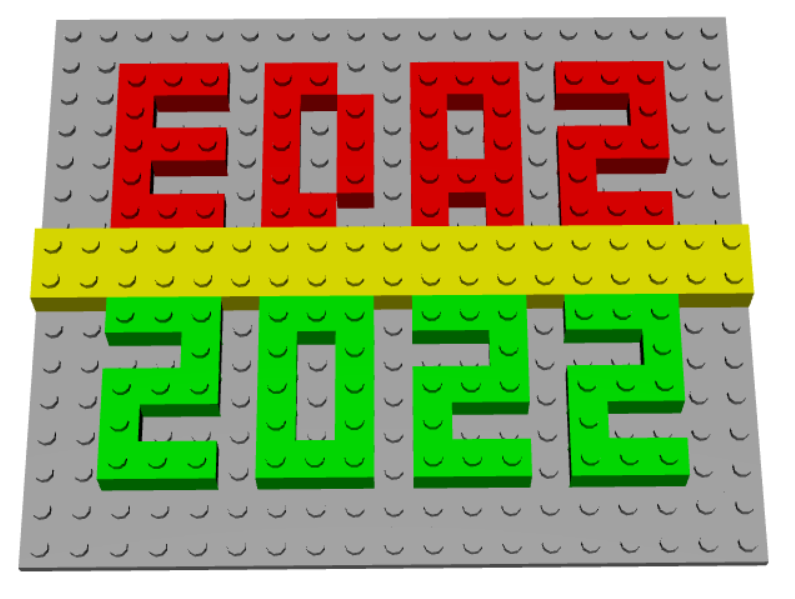
\includegraphics[scale=0.8]{imagens/EDA2_lego.PNG}
}
%---------------------------------------------------------------%
\author{
\textbf{Docente: }Vasco Pedro\\
\textbf{Grupo: } g121\\
\textbf{Discentes: } André Baião 48092, Gonçalo Barradas 48402\\
}
\date{Março 2022}
%---------------------------------------------------------------%

\begin{document}

\maketitle
\thispagestyle{empty}
\clearpage
%---------------------------------------------------------------%
\renewcommand{\contentsname}{Índice}
\thispagestyle{indice}
\tableofcontents
\clearpage
\setcounter{page}{1}
\section{Objetivo}
Com o intuito de avaliar os conhecimentos adquiridos pelos alunos foi proposto um trabalho que consiste na resolução do problema “Mosaics”. O trabalho consiste na elaboração de um programa, a representação da sua função recursiva e no cálculo das suas complexidades (temporal e espacial).

A resolução deste problema baseia-se na analise das sequências existentes num dado mosaico e no calculo do maior número de combinações possíveis de realizar com as peças permitidas.

\section{Descrição do algoritmo}

Para resolver este problema, o algoritmo deve conter 2 parte:
Na primeira parte recorre-se à análise linha a linha de forma a identificar as sequências de cores, podendo ocorrer um dos seguintes casos:
\begin{itemize}
    \item No primeiro caso é avaliado o primeiro valor e se este não for ".", então existe uma cor, começando uma sequência.
    \item No segundo caso se houver uma sequência seguida de um ".", então é calculado o valor das combinações possíveis e reiniciada a sequência.
    \item No terceiro caso é avaliado o último valor do mosaico, havendo dois pontos de avaliação:
    \begin{itemize}
        \item Se o valor actual for uma cor e se pertencer à sequência, então calcula-se o valor das combinações possíveis do tamanho da sequência mais um que corresponde à última peça.
        \item No caso de ser outro valor é calculado o valor das combinações dessa sequência e reiniciado o valor da mesma.
    \end{itemize}
    \item No quarto caso, o objectivo é avaliar qualquer posição do mosaico excluindo a primeira e a última posição. No caso de o valor ser igual ao penúltimo valor avaliado adiciona-se um ao tamanho da sequência, em qualquer outro caso é calculado o valor das combinações e reiniciado o valor da sequência.
\end{itemize}

A segunda parte tem como objectivo calcular as maneiras possíveis de realizar uma sequência utilizando as peças de lego permitidas.

Foi criado o método “possibleCombinations” que, para cada posição da sequência avalia quais as peças que podem ser utilizadas e calcula o número de combinações possíveis a realizar com essas peças. Este ciclo é executado n vezes conforme o número de sequência de cores que existam.


\section{Função Recursiva}
Dada uma sequência não vazia crescente de inteiros positivos \begin{equation*} B = (B_1 \, B_2 \ldots B_N) \end{equation*} , a função que calcula o número de maneiras diferentes que se pode fazer um determinado tamanho positivo\begin{equation*} i \end{equation*}é:\\
\begin{center}
\begin{equation*}
C_B(i) = \left \{
	    \begin{array}{l@{\quad}l}
	      1  & \mbox{se }\, i = 0          \\[8pt]
	      \displaystyle 
	      \sum_{N = 1 \land  \forall N : B_N \le i   }^{N} C_B(i-B_N)
		& \mbox{se }\, i > 0
	  \end{array} \right .
\end{equation*}
\end{center} 
A partir desta função, é possível obter um algoritmo iterativo :
\begin{lstlisting}
possibleCombinations(i)
    let C[0 ... i]   //novo array
    N = |T|             //Numero de peças
    m[0] = 1            //caso Base
    for x = 1 to i do
        j = 1
        while j <= N and B[j] <= x do
            C[x] = C[x] + C[x - B[j]]      //Caso recursivo
            j = j + 1
    return C[i]
\end{lstlisting}


\section{Calculo da Complexidade}

\subsection{Temporal}
Após a leitura dos dados necessários para a resolução do problema, vamos  analisar o mosaico,  que se encontra guardado numa matriz, começamos por inicializar 4 variáveis que nos vão auxiliar na resolução e análise do mosaico, cada um tem um custo de \verb|O(1)| logo \verb|4 x O(1)|, posteriormente começamos a analisar o mosaico. 

Para a análise do mosaico foram utilizados 2 ciclos, um interno e outro externo. No ciclo interno existem 5 condições de custo constante \verb|O(1)|, mas o ciclo tem um custo \verb|O(n)| onde \verb|n| é o numero de colunas do mosaico. O ciclo externo tem 1 condição que tem um custo constante \verb|O(1)|, um custo de \verb|O(m)| onde \verb|m| é o numero de linhas do mosaico e dentro deste ciclo ocorre também o ciclo interno.

Logo a análise do mosaico tem um custo de \verb|4 x O(4) + O(n x m) = O(|$\verb|n|^2$\verb|)| onde $\verb|n|^2$ é o numero de posições do mosaico.

A função "possibleCombinations" começa por inicializar uma matriz o que tem um custo constante \verb|O(1)|, depois de ser definido o caso base vamos é executado um ciclo que , tem um custo linear de \verb|O(n)| onde \verb|n| é o tamanho da sequência, neste ciclo existe um outro ciclo no qual existe uma condição que tem um custo de \verb|O(1)| , mas o ciclo tem um custo de \verb|O(m)| onde \verb|m| é o numero de peças diferentes.

Logo esta função tem um custo de :
\begin{center}
    \verb|O(1) + O(n) x O(m) x O(1) = O(|$\verb|n|^2$\verb|)|
\end{center}
Como na analise de dados a função "possibleCombinations" é chamada dentro dos dois ciclos a complexidade temporal do programa é:
\begin{center}
   \verb|O(|$\verb|n|^2$\verb|) x |\verb|O(|$\verb|n|^2$\verb|) = O(|$\verb|n|^4$\verb|)|
\end{center}

\subsection{Espacial}
Para calcular a complexidade espacial, foi necessário ter em conta a estrutura de dados utilizada para guardar os dados necessários para a realização do problema. Para guardar o mosaico foi utilizada uma matriz bidimensional, para inicializar a matriz foi necessário saber o número de linha e colunas, esses dois valores ocupam em memoria \verb|O(1)| cada. 

Para inicializar a matriz foi necessário saber o número de linha e de colunas do mosaico para determinar o espaço que a matriz iria ocupar em memoria. Seja n o numero de linhas do mosaico e m o numero de colunas do mosaico, a complexidade espacial desta matriz é \verb|O(n x m) = O(|$\verb|n|^2$\verb|)| 

Podemos concluir que a complexidade espacial do programa é:
\begin{center}
    \verb|O(1) + O(1) + O(|$\verb|n|^2$\verb|) = O(|$\verb|n|^2$\verb|)| 
\end{center}
\section{Comentários}
Durante a análise de dados, no caso de guardarmos todas as sequências do mosaico e só no fim calcularmos o numero de combinações possíveis melhoraríamos a complexidade temporal (\verb| O(|$\verb|n|^3$\verb|)| ) mas estaríamos a piorar a complexidade espacial.  (\verb| O(|$\verb|n|^2$\verb| + n)| )
\section{Conclusão}
Considerando a complexidade temporal e a complexidade espacial obtida podemos concluir que o desafio proposto foi concluído com sucesso. Tendo sido possível aplicar e consolidar os conhecimentos adquiridos ao longo da elaboração do trabalho.
\end{document}
